\documentclass[12pt, twocolumn]{article}
\usepackage[english]{babel}
\usepackage[utf8]{inputenc}
\usepackage{cite}
\usepackage{titling}
\usepackage{titlesec}

\usepackage[autostyle]{csquotes}
\usepackage{pgfgantt}
\raggedbottom
\titlespacing*{\section}{0pt}{0.5\baselineskip}{0.5\baselineskip}
\titlespacing*{\subsection}{0pt}{0.5\baselineskip}{0.5\baselineskip}
\titleformat*{\section}{\normalsize\bfseries}
\titleformat*{\subsection}{\small\bfseries}
\usepackage{hyperref}
\usepackage{calc}
\newlength{\myunitx}
\newlength{\autosizewidth}
\setlength{\autosizewidth}{\textwidth} % this allows you to change the value for autosizing
\newcommand*{\timeslots}{}
\ganttset{%
timeslots/.code args={#1,#2}{\setlength{\myunitx}{(\autosizewidth-\widthof{#2}-1em)/#1}
                 \renewcommand{\timeslots}{#1}\pgfkeys{pgfgantt/x unit=\myunitx}}
}

\usepackage{natbib}
\bibliographystyle{plainnat}

\usepackage[a4paper,margin=2cm,footskip=1.5cm]{geometry}
\usepackage{xspace}
\usepackage{fancyvrb}
\usepackage{lipsum}
\newcommand{\verbatimfont}[1]{\renewcommand{\verbatim@font}{\ttfamily#1}}
% Hyperref settings
\def\sectionautorefname{Section}
\def\subsectionautorefname{Section}
\def\subsubsectionautorefname{Section}

%% user defined macros
\newcommand{\project}{AFD}
\newcommand{\targetlanguage}{TypeScript}
\newcommand{\wptotal}{five}



% English
\newcommand{\cf}{\hbox{\emph{cf.}}\xspace}
\newcommand{\deletia}{\ldots [deletia] \ldots}
\newcommand{\etal}{\hbox{\emph{et al.}}\xspace}
\newcommand{\eg}{\hbox{\emph{e.g.}}\xspace}
\newcommand{\ie}{\hbox{\emph{i.e.}}\xspace}
\newcommand{\scil}{\hbox{\emph{sc.}}\xspace}
\newcommand{\st}{\hbox{\emph{s.t.}}\xspace}
\newcommand{\wrt}{\hbox{\emph{w.r.t.}}\xspace}
\newcommand{\etc}{\hbox{\emph{etc.}}\xspace}
\newcommand{\viz}{\hbox{\emph{viz.}}\xspace}

\newcommand{\todo}[1]{{\color{red}#1}}
\newcommand{\dl}[1]{\todo{For DL: #1}}
\newcommand{\eb}[1]{\todo{For Earl: #1}}

%% this is still a placeholder title
\title{Automatic Fix Detection} 

\author{David Landsberg \and Earl Barr}%


\date{%
}

%% document begins here
\begin{document}

\maketitle{}

\section{Executive Summary}
    
Software engineers spend most of their time maintaining, not writing, their programs. A critical part of maintenance involves discovering when a given program, previously demonstrated to be produce failures (violations of a given program specification), has been fixed. 
At present this is a manual process in which the program is 
inspected by the engineer and assessed as to whether a fix has occurred. Automation promises to improve the efficiency and effectiveness of this process, by delivering a report to the user which states that a method has been fixed with increased reliability, and in a smaller timescale than if performed manually. We call the problem of determining whether a fix has actually occurred in this way --- the \textit{automated fix detection problem} (AFDP). Solution to this problem 
has the potential to greatly improve the quality assurance of released software. It is this problem that our research will address. 
 

\section{Background and Context}
    Any solution to AFDP is expected to be a function of a failure's symptoms, such as stack traces and user/test reports. In large scale industrial projects, where software is developed using continual integration and deployment in conjunction with automatic verification and validation (V\&V), the need to solve this ``largely overlooked" problem is especially acute~\cite{Facebook1}.
This problem has recently been decomposed by Alshahwan \etal  into two subproblems: 

\begin{itemize}
\item  \emph{Failure grouping}, which associates groups of failures to the methods which generate them, and 

\item \emph{Proving a negative}, which determines when we can be confident failures will not recur (i.e. a fix has succeeded). 
\end{itemize}

We take up the challenge of solving these sub-problems. To group failures, we investigate methods of causal inference to assign each failure a root cause (WP1).  To prove a negative, we will investigate statistical change point detection methods to detect when a fix has succeeded in the presence of flaky tests (WP2). Combined, these offer a novel solution to the fix detection problem which is at once scalable and integratable into Industrial development process (WP3). 

Finally, solving AFDP facilitates the solution of a related problem which we describe as finding useful \textit{Fix-classifications and statistics}. Solution to this is critical at the software managerial level for determining areas for software development in the short term furture, providing a high-level description of how and what fixed have occurred dynamically over time (WP4).  We decompose this problem into two sub-problems:

\begin{itemize}
\item \textit{Fix-classification}, where fixes are put into a class which describes the fix. This can include fixes which solve an environmental or a resource dependent problem.

\item \textit{Fix statistics}, which describe the evolution of fixes over time.
\end{itemize}

Solution to the four problems thus provides, for any large scale software project, answers to four respective questions: which fixes have fixed which failures, which methods can be said to be fixed, what class of problem did the fixes fix, and how have fixes evolved. This gives us a comprehensive and automated treatment for understanding the evolution of fixed code, which in an implemented tool, will provide critical high level understanding of code for program managers. 

\section{Project Structure and Methodology}
    % project structure here
Our \wptotal{} work packages (WPs) seek to develop the project in the following ways. WP1 examines methods to treat the failure grouping problem. This progresses in concert with WP2 which examimes methods for solving the proving a negative problem. WP3 examines methods to treat the fix classification and statistical problem.  WP4 describes features of the tool which will be implemented as a consequence of the previous packages. 
See Figure~\ref{fig:gantt}.

The main high-level goal of \project{} is to build a  tool which can give comprehensive understanding about fixes, with the main desiderata being that these contribute to a debugging paradigm which is more effective and efficient at delivering information about fixes than if the user did not use the tool.  


    \begin{figure*}
    \noindent\resizebox{\textwidth}{!}{%
    \begin{ganttchart}
        [   vgrid, 
            hgrid,
            time slot format=isodate-yearmonth,
            compress calendar,
            group label font=\tiny ] {2018-10}{2021-10} 

        % \gantttitle{\project{} Work Flow}{12}\\
        \gantttitlecalendar{year, month}\\
        \ganttbar[bar/.append style={fill=blue}]{WP1: Failure Grouping}{2018-10}{2019-12}\\
        \ganttlinkedbar[bar/.append style={fill=red}]{WP2: Proving a Negative}{2019-06}{2020-05}\\
      %  \ganttlinkedbar[bar/.append style={fill=yellow}]{WP3: Fix Classification}{2019-12}{2020-12}\\
        \ganttlinkedbar[bar/.append style={fill=green}]{WP3: Taking Stock of Software}{2020-01}{2020-12}\\
         \ganttlinkedbar[bar/.append style={fill=cyan}]{WP4: Tool \& Deployment}{2020-05}{2021-10}
    \end{ganttchart}}
\caption{Expected Work flow for \project{}}
\label{fig:gantt}
\end{figure*}



\subsection*{WP1: Failure Grouping}
    
The failure grouping problem (FGP) is that of grouping failures to their likely causes (here assumed to be methods). Being able to tell which failures a method causes is key to being able to tell whether it is fixed.
 Thus far, a cutting edge method used in industry (namely, Facebook) by Alshahwan \etal is to use method identifiers (located at the top of stack traces) as the heuristic for grouping.
However, the designers of this technique propose this solution would be improved upon by applying techniques of causal inference.
They write "there has been much recent progress on causal inference \cite{Pearl} ... Therefore, the opportunity seems ripe for the further
development and exploitation of causal analysis as one technique for informing and understanding fix detection"~\cite{Facebook1}.

We take up the challenge left by Alshahwan \etal . For WP1, we propose to investigate different causal theories to solve the FGP. Here, we begin our development with 
the probabilistic measure of
causality due to Pearl~\cite{pearl2009,pearl2016causal}. We pick this particular theory because (as we shall see) there are simple and low-cost ways to estimate the value of the formula, and it opens the window to a number of different (potentially better) theories of causality.
Here, $C$ is a cause of the event $E$ when the following obtains:

\vspace*{-4.0mm}

\begin{equation}
    Pr(E | \mathit{do}(C)) > Pr(E | \mathit{do}(\neg C))
    \label{eq:pearl}
\end{equation}

The intuition is that causes raise the probability of their effects. 
Applied to FGP, we parse \autoref{eq:pearl} as follows:  $Pr(X|Y)$ reads "the
probability of $X$ given $Y$", $E$ is an event of a failure, and $C$ is the introduction of a given patch into the given
codebase. The operation $\mathit{do}(C)$ 
represents an external intervention that compels $C$ to obtain, whilst holding certain background factors fixed (in our case this is the rest of the codebase --- see Pearl for technical details~\cite{pearl2009}). Intuitively
then, $Pr(E | do(C))$ measures the probability that a
failure occurs upon the introduction of a given patch. Accordingly,
\autoref{eq:pearl} says that a
patch is a cause of the failure if the likelihood of the failure would have decreased had the patch not been introduced into the program.

A major question for our research is to estimate $Pr(E | do(C))$ and $ Pr(E |
do(\neg C))$. As a starting point, we envisage conducting a controlled experiment. Here, we assume i) we have a program together with its updated version, ii) that the updated version only differs from the original by a patch $C$, iii) that there is only one bug in the codebase, and iv) a fix for the bug repairs the method, and v) there is a test available  which can be run on both versions a given number of times  (in real-world testing scenarios we will not have to make all of these assumptions --- see~\autoref{sec:deployment}). Here, we propose $Pr(E|do(C))$  is estimated by the proportion of times the test results in failure in the updated version, and $Pr(E|do(\neg C))$  as the
proportion of times the test results in failure in the non-updated version. Note that the estimated probabilities might assume values anywhere in the interval $[0,1]$ --- depending on the presence of noise, indeterminism, flaky tests, and degree of unspecified behaviour. Accordingly, if \autoref{eq:pearl} holds, we say the method causes the given failure in that update for that test, thereby grouping the failure to the associated method as its cause. 

Pearl's theory is not enough. 
It is not guaranteed to handle (what Alshahawan calls) \textit{false grouping}~\cite{Facebook1}.
Accordingly, \autoref{eq:pearl} may include too many (or too few) causes in practice. To investigate this, we propose 
experimenting with different measures for the \textit{degree of causality} (which in our context may be said to measure \textit{error-causing degree}), such as $Pr(E | do(C)) - Pr(E | do(\neg C))$ and $Pr(E | do(C))/Pr(E | do(\neg C))$~\cite{pearl2009}, and saying causality obtains when the value given by the measure is over a given bound.  
Previous research has confirmed that different measures of causality perform very differently~\cite{eval}, suggesting a requirement to experiment with many different measures from the literature on A.I., fault localisation, and philosophy of science, of which there are hundreds~\cite{eval}.  

To summarise this WP, we propose investigating causal theories to solve FGP. A starting point is Pearl's theories, and different measures of causality must be examined, developed, and experimented upon to find one fit for purpose. 


 


\subsection*{WP2: Proving a negative}
    
Alshahwan \etal ask the following: ``how long  should we wait, while continually observing no re-occurrence of a failure (in testing or production)
before we claim that the root cause(s) have been fixed?"~\cite{Facebook1}  Here, we assume the root cause(s) of a failure have been estimated by the work of WP1. The famous \textit{proving a negative problem} rears its head here: How we can prove a negative (no more failures) in the absence of direct evidence to the contrary.  
Alshahwan \etal state that identifying the correct \textit{fix detection protocol}~\cite{Facebook1} provides the solution, and experiment with their own protocol within the Sapienz Team
at Facebook. Their protocol uses heuristics and a finite state machine, but emphasize they ``do not claim it is the only possible protocol, nor that it is best among alternatives".  Accordingly, In this WP we propose the investigation of principled alternatives.

To begin our development, we propose to answer Alshawan's question above directly: We wait until we can claim a fix has occurred, i.e. when the error-causing behaviour of the method has diminished. 
Our answer is made precise as follows. 
We let the \textit{error causing behaviour} of a given method be a time series T = $t_1, t_2, \dots, t_n$, where each datapoint is an error-causing degree for a given failure group (as per WP2) over a given period. Let T1 = $t_1, t_2, \dots , t_k$ and T2 = $t_{k+1}, t_{k+2}, \dots , t_n$ be two adjacent time series splitting T.  Following the standard definition of changepoint detection, a \textit{changepoint} is detected for T1 and T2 if T1 and T2 are shown to be drawn from a different distribution according to a given hypothesis testing method~\citep{Aminikhanghahi, arXiv:1411.7955}.
We detect that some \textit{fix}/\textit{bug} has been introduced into T2 since T1, if i) a changepoint is detected for T1 and T2 and ii) the average error causing degree in T2 is smaller/larger than the average error causing degree in T1. Finally, we say the the error-causing behaviour of the method has \textit{diminished} when a fix is detected.

To illustrate the setup, consider~\autoref{f1}, which represents a time series of real-valued datapoints. Let T1 be the series before the vertical green line and T2 the series after. Already, our setup could be used to say some fix has been introduced into T2 since T1. It then remains to find the precise point where the fix was introduced. This is done by applying a changepoint detection method (CDM). In general, CDMs try to identify exact times (\textit{changepoints}) when the probability distribution of a stochastic process or time series can be confidently said to change. 
Ideally, we would apply a CDM which identifies the changepoint with the datapoint indicated by the green line in~\autoref{f1}.  
Research into CDMs is a large and well-developed area~\citep{Aminikhanghahi, arXiv:1411.7955}, and have been applied successfully to solve similar problems to FDP in continuous code deployment~\cite{arXiv:1411.7955}. Key differences between CDMs include where they locate changepoints, and how scalable the technique is. 





\begin{figure}[t!]
  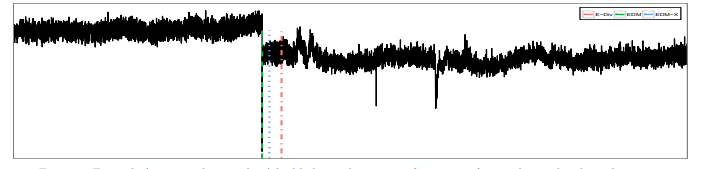
\includegraphics[width=\linewidth]{cp_z.png}
  \caption{Time Series with Change Point.}
  \label{f1}
  
\vspace*{-0.6cm}

\end{figure}




\subsection*{WP3: Tool Deployment} %% \todo{possibly merge with WP2}
    Software managers want to know several additional statistics and features about the fixes to help them manage and understand their code, over and above what is provided for by WP1 and WP2. Investigating and developing these statistics and features will be the project of WP3. We divide the project into a \textit{quantitive} sub-project, and \textit{qualitative} sub-project, as follows.

We first discuss the quantitive sub-project. This will include finding appropriate statistical measures for quantities of interest to a software manager, and developed as a function of the time series of error-causing propensities developed in WP1 and WP2. Basic statistics which answer the following questions will be of value, and can be decomposed into descriptive statistics (which describe how code development has behaved in the past) and, where possible, predictive statistics (which forecast how code development will continue in the future). Questions that can be given a statistical answer here include (but are not limited to) i) how many (or what is the rate of) fixes (or new bugs) which have taken place (or are to be expected) over a given time period, ii) what's the expected likelihood a type of bug will recur, iii) how many times has a fix been attempted for a given method, how many have worked, vi) how stable is the development of the code overall. Accordingly, in the first part of the workpackage we will develop and investigate these statistical measures. We expect these measures to fall within a range of elementary measures, to more sophisticated ones.  

We now discuss the qualitative sub-project. 
This includes correctly classifying a given fix into its fix type. This involves i) correct bug classification (to know what bug was fixed), ii) correctly associating each fix with a bug, and iii) the type of fix repaired the bug.
WP1 and WP2 solve ii), and methods exist at bug classification to help solve i), and can involve test mining engineering reports, or testing of the program before and after the given fix~\cite{6245635}. However, to our knowledge no work has been done at iii). Here, we (at least) want to know whether the fix fixed the bug in an efficient/inefficient, effective/ineffective, syntactically simple/complex way; paving the way for a large dictotomy table of different types of fix. For instance, a fix may have added an undue amount of runtime to a project, may have only been effective at solving a certain proportion of failures, and may involve a lot of complex code involving the addition of pointers or other new types of structures to the code. Any project manager will want to know the classes of this sort to which a fix belongs.  



%\subsection*{WP4: Fix Classification}
 %   
We will implement our tool in a usable piece of software which can be integrated in several different scenarios. 
To illustrate, we discuss three example integration scenarios; with the Sapienz tool, FBlearner, and canary testing. We then discuss the development of our techniques.

The first area of deployment is alongside the Sapienz tool, which
has been integrated alongside Facebook's production development process Phabricator~\citep{Facebook1} to help identify faults. Accordingly, our methods could be integrated alongside Sapienz to help detect fixes made as a consequence of testing. 
The second area of deployment is alongside FBLearner, a Machine Learning (ML) platform through which most of Facebook's ML work is conducted. In FBlearner there is an existing fix detection workflow stage~\citep{Facebook1}, which involves using reinforcement learning to learn to classify faults and fixes. Accordingly, our methods could be integrated in the fix classification stage. 

The third area of deployment is alongside Facebook's canary testing/rolling deployment process for mobile devices. Canary releasing slowly rolls out changes to a small subset of users before rolling it out to the entire infrastructure. Facebook uses a strategy with multiple canaries (versions)~\cite{7883285,canaryrelease}.
In practice, data about different canaries could be used to form part of the dataset used for our fix detection methods. Namely, if an update is deployed in one cluster but not another, we will have important data about which failures are caused by which updates and for which methods. 

Development of this work package involves making a tool which is  sufficiently general as to fit into any one these deployment scenarios, and is independent of the underlying language of the project under test. 


\subsection*{WP4: Taking Stock of your Software}
    
We will implement our tool in a usable piece of software which can be integrated in several different scenarios. 
To illustrate, we discuss three example integration scenarios; with the Sapienz tool, FBlearner, and canary testing. We then discuss the development of our techniques.

The first area of deployment is alongside the Sapienz tool, which
has been integrated alongside Facebook's production development process Phabricator~\citep{Facebook1} to help identify faults. Accordingly, our methods could be integrated alongside Sapienz to help detect fixes made as a consequence of testing. 
The second area of deployment is alongside FBLearner, a Machine Learning (ML) platform through which most of Facebook's ML work is conducted. In FBlearner there is an existing fix detection workflow stage~\citep{Facebook1}, which involves using reinforcement learning to learn to classify faults and fixes. Accordingly, our methods could be integrated in the fix classification stage. 

The third area of deployment is alongside Facebook's canary testing/rolling deployment process for mobile devices. Canary releasing slowly rolls out changes to a small subset of users before rolling it out to the entire infrastructure. Facebook uses a strategy with multiple canaries (versions)~\cite{7883285,canaryrelease}.
In practice, data about different canaries could be used to form part of the dataset used for our fix detection methods. Namely, if an update is deployed in one cluster but not another, we will have important data about which failures are caused by which updates and for which methods. 

Development of this work package involves making a tool which is  sufficiently general as to fit into any one these deployment scenarios, and is independent of the underlying language of the project under test. 
 

\section{Resources and Management}
    The activies in the WPs will need to be closely integrated. The foundational work developed in each of the work packages
will strongly influence the outcomes of the other WPs. Given the novelty of the work, alternative solutions will be developed if others seem impractical
or unscaleable. 

We now discuss development issues. To develop WP1, we will need an experimental framework where we can evaluate the performance of different causal measures on given benchmarks using standard IR measures (such as accuracy, precision, recall, and F-scores). We will evaluate the measures on different testing scenarios which do not make many of the restrictive assumptions outlined in 2.1. For instance, if i) is not true we need to perform fault localisation using a causal measure on the updated program alone (using a given fault localisation setup~\cite{eval}). If ii) or iii) are not true we will need to employ measures empirically demonstrated to perform well in the presence of noise~\citep{pearl2016causal}. 

The development of WP2 will include an experimental comparison of different CDMs, testing for effectiveness and scalability when employed at the fix detection task. To measure effectiveness, we use standard IR methods~\citep{Aminikhanghahi, arXiv:1411.7955}. To measure scalability, we will measure practical runtime on representative benchmarks. This work is made feasible insofar as many CDMs are already implemented, known to scale well, and can be used in an "online" contexts involving continuous real-time streams of datapoints.\footnote{\scriptsize{\url{http://members.cbio.mines-paristech.fr/~thocking/change-tutorial/RK-CptWorkshop.html}}} 

The development of WP3 will include research into time series data analysis, and also methods used for stock market analysis. In an ideal case, we would expect a research output of a program analysis tool which could display time series analyses in the same way as a trading tool might. Here the data analysed would be in terms of code performance as opposed to stock performance.  Given the potential for modularity of such a tool, with many different stacked components, the development of this project would allow the production of anywhere between a lightweight and a heavyweight tool.

%% almost word for word from LUCID
\project{} will be based at UCL, London campus. Project leads will be EB and DL with an RA also
based at UCL\@. The RA's career development will be fostered through giving presentations,
organising workshops, and visiting industrial partners. The RA will be encouraged to present
work at internal seminars and international conferences. The RA will learn community and networking
skills by organising and chairing workshops at the host university on \project{} from the
prospective of expertise channels. 

%Visits to Microsoft will allow the establishment of personal and
%professional connections with industrial researchers. Visits to Chalmers in Sweden will foster
%personal and professional connections with language-based security researchers. 


\section{Timeliness and Novelty}
    Automated fix detection is distinct from automated error detection, which has a large area of study, and implemented commerical tools (such as Airbrake~\footnote{\url{https://airbrake.io/}}) Automated fix detection is an entirely new area of study, and will also require integration into pre-existing tools. As of this present moment, no-one has yet attempted to create
an automated fix detection method which combines these methods into a tool. This would not be
only part of the novelty of our work. Most importantly we propose to create a system which sits `on
top' of any existing industrial scale software project, and rely on particular uses of program languages or managerial styles. This makes the methods developed in the project entirely general. 



\section{Academic Impact}
    Automated fix detection research fits within the field of software engineering (SE). The UK is considered a strong contributor to this field, therefore this project will contribute to maintaining UK's top position in this area. 

As software systems grow in scale and complexity, it faces additional challenges when trying to assertain its properties. This project will attack this challenge by developing methods which can determine properties relevant to fixes. 
The project will have a significant impact in software engineering by identitying new lines of research for software development methods involving fix detection. We also expect impact to be had in areas related to the application of AI (given practical applications of methods of causal inference in WP1), and the application of statistical methods (such as change point detection of WP2), bug/fix ontologies (WP3), quality assurance statistics (WP3), and programming tools (WP4). 
Outcomes of the project include submissions to the top software engineering conferences and journals. These include ICSE, FSE, ISSTA, and TSE.  


\section{National Importance}
    The software sector is a substantial contributor to UK economic growth. Engineering-UK reports: "\textit{software, IT and telecoms together generated 4.2\% of UK gross value added in 2011 and provided 885,000 jobs. There are 107,000 software businesses, and the UK is the world's number two exporter of telecoms services (£5.4 billion) and number three in computer services (£7.1 billion) and information services (£2 billion)"}.\footnote{\url{https://www.engineeringuk.com/media/1466/enguk-report-2015-interactive.pdf}}

To contribute to this, our proposed research will produce new disruptive technologies, consistent with the EPSRC's deliver plan of 17-2019/20. Our project aims to offload the laborious process of fix detection to an automatic process. Success in this area will thus challenge the status quo of software development. Developers will be able to spend more time on other tasks, making them more productive and subsequently facilitating further economic growth. 

Finally, the UK is already world-leading in software engineering. However, at
present there are no UK researchers active in the field of automated fix detection. Our project would put the UK at the forefront of such research. In addition, as 
software engineering is considered an area of high priority growth by
EPSRC, our project will offer a bridgehead to work of national and international importance.


\bibliographystyle{ACM-Reference-Format}
\bibliography{sample-bibliography}

\end{document}
